\subsection{Encontrando matriz banda p,q}

Como dice el enunciado, cada una de las $2n$ juntas aporta 2 nuevas ecuaciones. El sistema lineal resultante tiene por lo tanto $4n$ ecuaciones con $4n$ incógnitas.
Intuitivamente lo que buscamos es que los números identificadores de las variables que actúan sobre una misma junta sean cercanos entre sí (Eso implica una buena numeración sobre los links de la estructura,
que respresentarán las variables).
Al mismo tiempo queremos que las juntas en donde interviene un determinado link no queden lejos entre sí (Eso implica una buena numeración sobre las juntas de la estructura, que respresentarán las filas).
En primer lugar, para encontrar la matriz banda $B_{p,q}$ dibujamos un puente Pratt Truss de 8 secciones y miramos fijamente la estructura tratando de realizar deducciones al respecto.

\begin{figure}[!h]
	\begin{center}
		  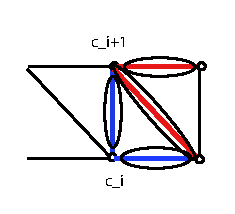
\includegraphics[keepaspectratio]{Imagenes/im_3.pdf}
		  \caption{Cada nuevo par de juntas introduce 4 nuevas fuerzas}
		  \label{fig:contra1}
	\end{center}
\end{figure}
\FloatBarrier

Si miramos a las juntas de a pares verticales: \{c1,c2\}, \{c3,c4\}, \ldots podemos advertir que por cada nuevo par se presentan 4 nuevas fuerzas. A su vez, cada una de las juntas tiene asociada 2 ecuaciones
del sistema (Uno para las fuerzas horizontales y otro para las verticales). Entonces podemos pensar que se introducen 4 nuevas variables cada 4 ecuaciones (1 por ecuación). Por lo tanto, es razonable pensar
que con la numeración correcta podemos llegar a obtener una matriz banda $B_{p,q}$, ya que los coeficientes distintos de cero se concentrarían alrededor de la diagonal. Además, un determinado link solo actúa 
sobre 2 juntas. Indudablemente debemos aprovechar este hecho para establecer el valor $p$ de nuestra matriz. Una numeración razonable consiste en aplicarle (tanto a los links como a las juntas) valores en
forma creciente de izquierda a derecha, y de abajo hacia arriba, tal como está representado en el siguiente diagrama:

\begin{figure}[!h]
	\begin{center}
		  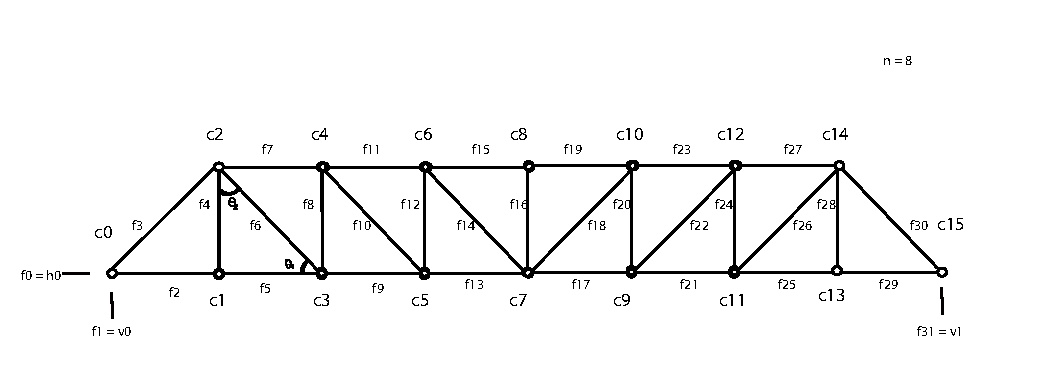
\includegraphics[keepaspectratio]{Imagenes/im_1.pdf}
		  \caption{Numeración para puente de 8 secciones}
		  \label{fig:contra1}
	\end{center}
\end{figure}
\FloatBarrier

Con dicha numeración, renombrando $junta_{i}=c_{i}$ y $link_{j}=f_{j}$, las primeras 6 ecuaciones (correspondientes a las primeras 3 juntas) del sistema lineal obtenido serían:

Ecuación 0: $c_{0} \ = 1*h_{0} + 0*v_{0} + 1*f_{2} + cos(\theta_{1})*f3 + 0*f_{4} + 0*f{5} + 0*f{6} + 0*f_{7} \ldots$

Ecuación 1: $c_{0} v = 0* h_{0} + 1*v_{0} + 0*f_{2} + sen(\theta_{1})*f3 + 0*f_{4} + 0*f{5} + 0*f{6} + 0*f_{7} \ldots$

Ecuación 2: $c_{1} \ = 0* h_{0} + 0*v_{0} - 1*f_{2} + 0*f3 + 0*f_{4} + 1*f{5} + 0*f{6} + 0*f_{7} \ldots$

Ecuación 3: $c_{1} v = 0* h_{0} + 0*v_{0} - 0*f_{2} + 0*f3 + 1*f_{4} + 0*f{5} + 0*f{6} + 0*f_{7} \ldots$

Ecuación 4: $c_{2}  \ = 0* h_{0} + 0*v_{0} - 0*f_{2} - sen(\theta_{2})*f3 + 0*f_{4} + 0*f{5} + sen(\theta_{2})*f{6} + 1*f_{7} \ldots$

Ecuación 5: $c_{2}v  \ = 0* h_{0} + 0*v_{0} - 0*f_{2} - cos(\theta_{2})*f3 - 1*f_{4} + 0*f{5} + cos(\theta_{2})*f{6} + 0*f_{7} \ldots$

~

Los siguientes pares de ecuaciones (luego de analizar las primeras tres juntas, y antes de llegar a las de la mitad de la estructura) comparten una especie de patrón. Notemos en primer lugar que los números
de las ecuaciones correspondientes a analizar la junta $c_{i}$ son $2*i$, correspondiente al plano horizontal y $2*(i+1)$, correspondiente al plano vertical. Además debemos considerar también si la junta es 
inferior o superior.

Si $c_{i}$ es junta inferior, entonces:

Ecuación $(2*i)$ \ \ \ \ \  : $c_{i} = -1*f_{2i-1} - cos(\theta_{1})*f_{2i} + 0*f_{2i+1} + 0*f_{2i+2} + 1*f_{2i+3}$   

Ecuación $(2*i+1)$ : $c_{i} v = sen(\theta_{1})*f_{(2i+1)-1} + 0*f_{2i+1} + 1*f_{(2i+1)+1} + 0*f_{(2i+1)+2} + 0*f_{(2i+1)+3}$

~

Si por el contrario, $c_{i}$ es junta superior entonces:

Ecuación $(2*i)$ \ \ \ \ \  : $c_{i} = -1*f_{2i-1} + 0*f_{2i} + 0*f_{2i+1} + sen(\theta_{2})*f_{2i+2} + 1*f_{2i+3}$   

Ecuación $(2*i+1)$ : $c_{i} v = -1*f_{(2i+1)-1} + 0*f_{2i+1} - cos(\theta_{2})*f_{(2i+1)+1} + 0*f_{(2i+1)+2} + 0*f_{(2i+1)+3}$

~

Las ecuaciones de las juntas del medio: $c_{n-1}$ la inferior y $c_{n}$ la superior deben ser planteadas aparte ya que son distintas al resto:

~

Inferior:

Ecuación $(2(n-1))$ : $c_{n-1} = -1*f_{2(n-1)-1} - cos(\theta_{1})*f_{2(n-1)} + 0*f_{2(n-1)+1} + 0*f_{2(n-1)+2} + 1*f_{2(n-1)+3} + cos(\theta_{1})*f_{2(n-1)+4}$ \\  

Ecuación $(2n-1)$ : $c_{n-1} v = -sen(\theta_{1})*f_{(2n-1)-1} + 0*f_{2n-1} + 1*f_{(2n-1)+1} + 0*f_{(2n-1)+2} + sen(\theta_{1})*f_{(2n-1)+3}$

~

Superior:

Ecuación $(2n)$ : $c_{n} = -1*f_{2n-1} + 0*f_{2n)} + 0*f_{2n+1} + 0*f_{2n+2} + 1*f_{2n+3}$ \\  

Ecuación $(2n+1)$ : $c_{n} v = -1*f_{(2n+1)-1} + 0*f_{2n+1} + 0*f_{(2n+1)+1} + 0*f_{(2n+1)+2} + 0*f_{(2n+1)+3}$

~

Los siguientes pares de ecuaciones vuelven a compartir un patrón (al igual que en la primera parte). Esto sucede para todos los pares restantes, con excepción del último:  

~

Si $c_{i}$ es junta inferior, entonces:

Ecuación $(2*i)$ \ \ \ \ \  : $c_{i} = -1*f_{2i-1} + 0*f_{2i} + 0*f_{2i+1} + 0*f_{2i+2} + 1*f_{2i+3} + cos(\theta_{1})*f_{2i+4}$   

Ecuación $(2*i+1)$ : $c_{i} v = 0*f_{(2i+1)-1} + 0*f_{2i+1} + 1*f_{(2i+1)+1} + 0*f_{(2i+1)+2} + sen(\theta_{1})*f_{(2i+1)+3}$

~

Si por el contrario, $c_{i}$ es junta superior entonces:


~

Finalmente, quedan analizar por separado las últimas 3 juntas: el par \{$c_{2n-3},c_{2n-2}$\} y $c_{2n-1}$: \\

Ecuación $(2(2n-3))$ \ \ : $c_{2n-3} = -1*f_{2(2n-3)-1} + 0*f_{2(2n-3)} + 0*f_{2(2n-3)+1} + 0*f_{2(2n-3)+2} + 1*f_{2(2n-3)+3} $ \\

Ecuación $(2(2n-3)+1 = 4n-5)$ : $c_{2n-3} v = 0*f_{(4n-5)} + 1*f_{(4n-5)+1} + 0*f_{(4n-5)+2} $ \\

Ecuación $(2(2n-2))$ \ \ : $c_{2n-2} = -sen(\theta_{2})*f_{2(2n-2)-2} - 1*f_{2(2n-2)-1} + 0*f_{2(2n-2)} + 0*f_{2(2n-2)+1} + sen(\theta_{2})*f_{2(2n-2)+2} $ \\

Ecuación $(2(2n-2)+1 = 4n-3)$ : $c_{2n-2} v = -cos(\theta_{2})*f_{(4n-3)-3} + 0*f_{(4n-3)-2} - 1*f_{(4n-3)-1} + 0*f_{(4n-3)} + cos(\theta_{2})*f_{(4n-3)+1} $ \\

Ecuación $(2(2n-1))$ \ \ : $c_{2n-1} = -1*f_{2(2n-1)-1} - cos(\theta_{1})*f_{2(2n-1)} + 0*f_{2(2n-1)+1} + 0*f_{2(2n-1)+2}$ \\

Ecuación $(2(2n-1)+1 = 4n-1)$ : $c_{2n-1} v = sen(\theta_{1})*f_{(4n-1)-1} + 1*f_{(4n-1)} + 0*f_{(4n-1)+1} + 0*f_{(4n-1)+2}$ \\


\begin{figure}[!h]
	\begin{center}
		  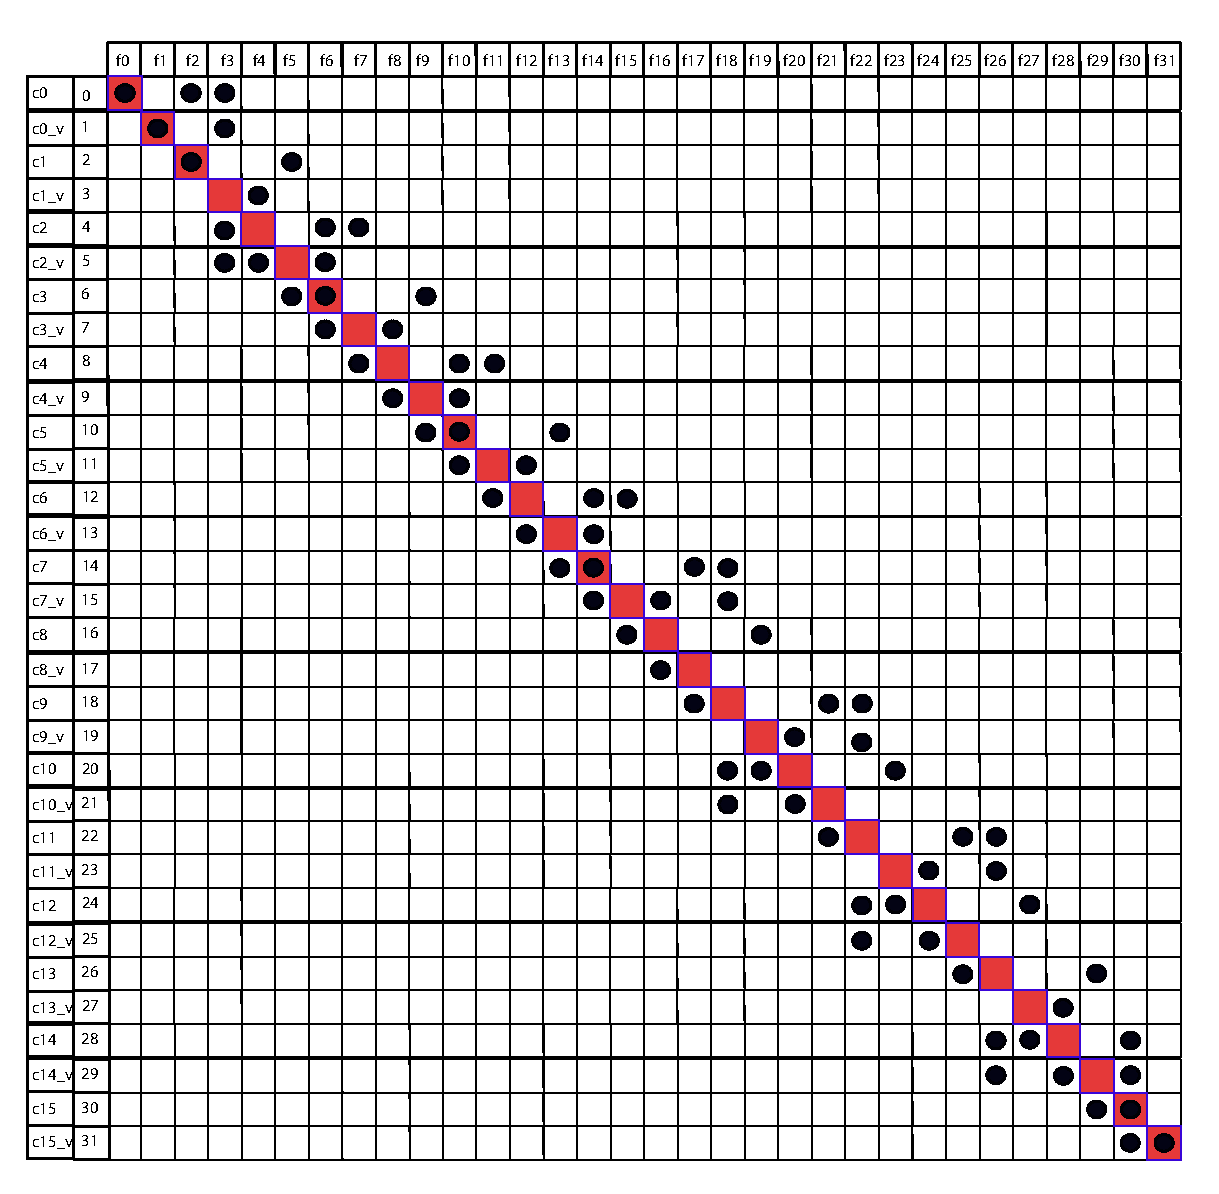
\includegraphics[scale=0.5]{Imagenes/im_2.pdf}
		  \caption{Esquema de matriz a partir del sistema de ecuaciones}
		  \label{fig:contra1}
	\end{center}
\end{figure}
\FloatBarrier

Al mirar el esquema de la matriz podemos llegar a clasificar rápidamente a la matriz como banda 3,4. Tratemos de analizar un poco este hecho:

Sea $b$ nuestra matriz. 
La mitad izquierda de la banda, también conocida como $p$, está relacionada con la mayor distancia entre una fila $i$, y una fila $j$, con $j \geq i$ para 
las cuales el $link_{i}$ interviene en la ecuación de la fila $j$. Por lo tanto, si llamamos $p$ a esta distancia observamos que:

- $b_{j,j-p} \neq 0$. Justamente, $j-p = i$, y habíamos dicho que $link_{i}$ interviene en dicha ecuación.

- Sea $h$ una fila tal que $h \neq j$. Entonces, el índice de la columna más a la izquierda que tiene un coeficiente $\neq 0$ es mayor o igual a (h-p).

\begin{figure}[!h]
	\begin{center}
		  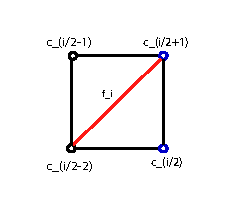
\includegraphics[scale=1.5]{Imagenes/im_4.pdf}
		  \caption{Explicación de la mitad izquierda de la banda: \emph{p}}
		  \label{fig:contra1}
	\end{center}
\end{figure}
\FloatBarrier

En el caso de nuestro puente, las juntas que presentan esta máxima distancia \emph{p} son aquellas como las que muestra la 
figura, pintadas en azul: Par alineado verticalmente perteneciente a la segunda mitad del puente.  

\begin{figure}[!h]
	\begin{center}
		  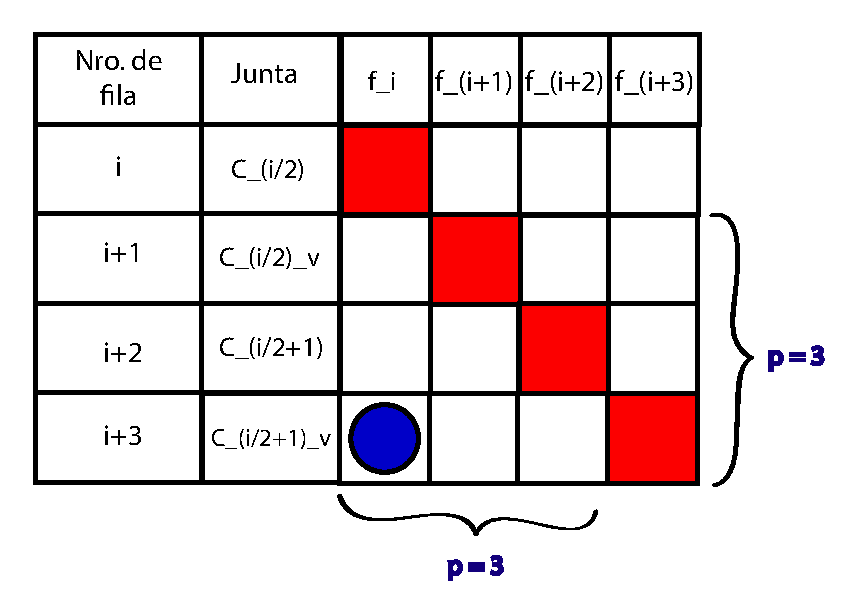
\includegraphics[scale=0.5]{Imagenes/im_5.pdf}
		  \caption{Explicación de la mitad izquierda de la banda: \emph{p}}
		  \label{fig:contra1}
	\end{center}
\end{figure}
\FloatBarrier

Tal como vemos en la figura 5, el coeficiente que acompaña a $f_{i}$ es distinto de cero en la ecuación $i+3$. Esto determina
una banda izquierda $p \leq 3$. Sin embargo, para ningún par de ecuaciones se cumple $p > 3$. Por lo tanto, podemos concluir que $p=3$.

~

La mitad derecha de la banda, conocida como $q$, está relacionada con el link de mayor numeración que interviene en la ecuación
de una junta. Profundizando un poco, al analizar la ecuación $i$, la 
diferencia entre la mayor columna $j$ y la columna $i$ (con $j \geq i$ tal que $b_{i,j} \neq 0$)
determina la mitad derecha de la banda para dicha ecuación. La mayor de estas diferencias para todas las filas determina $q$.

\begin{figure}[!h]
	\begin{center}
		  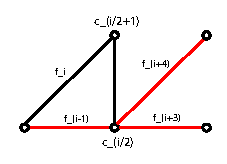
\includegraphics[scale=1.5]{Imagenes/im_6.pdf}
		  \caption{Explicación de la mitad derecha de la banda: \emph{q}}
		  \label{fig:contra1}
	\end{center}
\end{figure}
\FloatBarrier

Tal como muestra el esquema, esta máxima diferencia se produce en las ecuaciones horizontales pertenecientes a las juntas
inferiores de la segunda mitad del puente. 

\begin{figure}[!h]
	\begin{center}
		  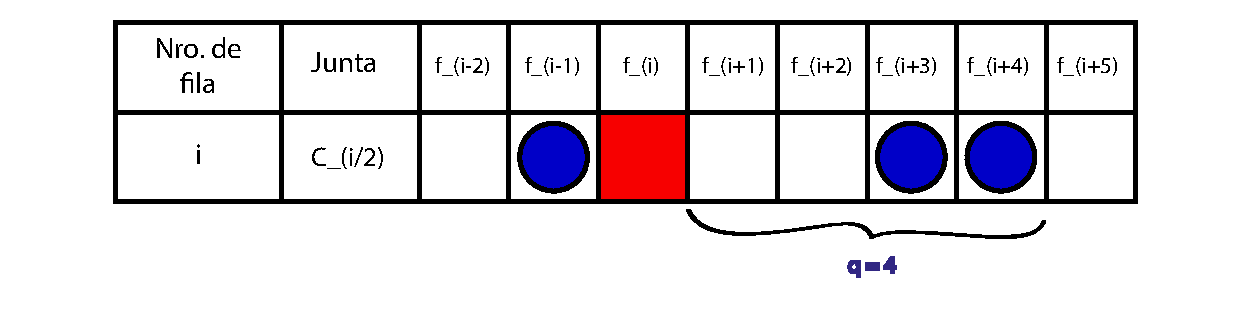
\includegraphics[scale=0.5]{Imagenes/im_7.pdf}
		  \caption{Explicación de la mitad derecha de la banda: \emph{q}}
		  \label{fig:contra1}
	\end{center}
\end{figure}
\FloatBarrier

Al analizar la fila $i$, perteneciente a la ecuación horizontal de la junta $\frac{i}{2}$, el link de mayor numeración que
interviene en la ecuación es $i+4 \Rightarrow \ q \geq 4$. Sin embargo, para ninguna ecuación esta diferencia es mayor que 
4, por lo que podemos concluir que $q=4$.

